\section{Connectivity}

\subsection{Bounding the Edges}

\begin{theorem}\label{thm:graph-edge-bounds}
  Let \(G\) be a simple graph on \(n\) vertices. If \(G\) has \(k\) components,
  then the number of edges of \(G\), denoted \(m\), satisfies
  \[ n-k \leq m \leq \frac{(n-k)(n-k+1)}{2} \]
\end{theorem}

\begin{proof}
  First, we will prove the lower bound. Claim that, for a connected graph \(G\)
  with \(n\) vertices, \(|E(G)| = m \geq n-1\). We will show this by induction on \(n\).
  Let \(m_j\) denote the number of edges in a graph with \(j\). When 
  \(n = 1\), then we have 0 edges. Hence, \(m_1 \geq n-1 = 1 - 1 = 0\) satisfies
  in the base case. Let us assume that the \(m_{n-1} \geq (n-1) - 1 = n-2\). We
  will now show for general case of \(n\) vertices, consider the following.
  \[
  \begin{aligned}
    m_n & \geq m_{n-1} + 1 & \qquad\text{[Add vertex and add one edge]} \\ 
        & \geq (n - 2) + 1 \\ 
        & \geq n - 1
  \end{aligned}
  \]
  Now, let us assume that \(G\) has \(k\) components and let \(n_i\) denote the
  number of vertices in the \(i\)-th component. Notice that \(n_1 + n_2 + \cdots
  + n_k = n\). Then, the minimum of the entire graph would be the sum of the
  minimum of each component.
  \[
  \begin{aligned}
    m \geq (n_1 - 1) + (n_2 - 1) + \cdots + (n_k - 1) &= n-k
  \end{aligned}
  \]

  Now, we will prove the upper bound. Assume that each component of \(G\) is a
  complete graph. Compare two components \(C_i\) and \(C_j\) with \(n_i\) and
  \(n_j\) vertices where \(n_i \geq n_j > 1\). Consider replacing \(C_i\) and
  \(C_j\) with complete graphs with \(n_i + 1\) and \(n_j - 1\) vertices, 
  respectively. Then, the number of vertices is the same and the change in
  number of edges is as follows.
  \[
  \begin{aligned}
    \binom{n_i + 1}{2} + \binom{n_j - 1}{2} - \left[\binom{n_i}{2} + \binom{n_j}{2}\right]
      &= \frac{(n_i+1)n_i}{2} + \frac{(n_j-1)(n_j-2)}{2} 
        - \left[\frac{n_i(n_i-1)}{2} + \frac{n_j(n_j-1)}{2}\right] \\ 
      &= \frac{(n_i + 1)n_i - (n_i - 1)n_i}{2} +
        \frac{(n_j - 2)(n_j - 1) - n_j(n_j - 1)}{2} \\ 
      & = \frac{2n_i}{2} + \frac{(-2)(n_j-1)}{2} \\ 
      & = n_i - n_j + 1 > 0
  \end{aligned}
  \]
  Repeat this argument until \(n_1 = n-k+1\) and the rest has only 1 vertex.
  Then, the maximum number of edges is
  \[ \binom{n-k+1}{2} = \frac{(n-k+1)(n-k)}{2} \]
\end{proof}

\begin{corollary}
  Any simple graph with \(n\) vertices and more than \(\frac{(n-1)(n-2)}{2}\)
  edges is connected.
\end{corollary}

\begin{proof}
  Assume that \(G\) is a disconnected graph. That is, suppose that \(k\) denotes 
  the number of components of \(G\), then \(k \geq 2\). Then, the number of 
  edges in \(G\), denoted \(m\) is bounded by
  \[ m \leq \frac{(n-2)(n-1)}{2} \]
  by Theorem \ref{thm:graph-edge-bounds}. If \(k\) is greater than 2, then the 
  upper bound decreases. Thus, if \(m > \frac{(n-2)(n-1)}{2}\), then \(G\) must be connected.
\end{proof}

\subsection{Distance and Diameter}

\begin{definition}[Distance]
  The \textit{distance} between vertices \(u\) and \(v\) in \(G\), denoted
  \(d(u, v)\), is the smallest length of a \(u - v\) path.
\end{definition}

\begin{definition}[Diameter]
  The \textit{diameter} of \(G\), denoted \(\diam(G)\), is the biggest distance
  between any two vertices of \(G\).
\end{definition}

\begin{definition}[Geodesic]
  A \(u - v\) path of length \(d(u, v)\) is called a \(u - v\)
  \textit{geodesic}.
\end{definition}

\begin{theorem}\label{thm:graph-diameter}
  Let \(G\) be a connected graph of order \(n\). If 
  \[ \deg(u) + \deg(v) \geq n-1 \]
  for every two non-adjacent vertices \(u, v \in V(G)\), then \(G\) is connected
  and \(\diam(G) \leq 2\).
\end{theorem}

\begin{proof}
  Let \(u, v \in V(G)\). If \(u\) and \(v\) are not adjacent, then \(d(u, v) = 2\) due to the
  Pigeonhole Principle. Recall that the maximum degree a vertex can have is
  \(n-1\). So, if the sum of two vertices' degrees is greater than \(n-1\), then
  there must be some vertices that show up in both neighborhoods. Hence, the
  distance of 2 can be derived as a path from \(u\) to a shared neighbor and
  then \(v\). Otherwise, \(u\) and \(v\) are adjacent and \(d(u, v) = 1\). Thus,
  the maximum distance between any two vertices is 2. Therefore, we have that 
  \(\diam(G) \leq 2\).
\end{proof}

\begin{remark}
  If \(G\) is a complete graph, then \(d(u, v) = 1\) for every pair of edges
  \(u, v \in V(G)\). In that case, \(\diam(G) = 1 \leq 2\).
\end{remark}

\subsection{Maximum and Minimum Degrees}

\begin{definition}
  For a graph \(G\), \(\delta(G)\) denotes the minimum degree and
  \(\Delta(G)\) denotes the maximum degree in \(G\).
\end{definition}

\begin{corollary}
  If \(G\) is a graph of order \(n\) such that for any \(u, v \in G\) with
  \(\delta(G) \geq \frac{n-1}{2}\), then \(G\) is connected.
\end{corollary}

\begin{proof}
  Notice that if \(\delta(G) \geq \frac{n-1}{2}\), then \(\deg v \geq
  \frac{n-1}{2}\) for any \(v \in V(G)\). Then, we have that
  \ref{thm:graph-diameter}, we have that
  \[ \deg u + \deg v \geq \frac{n-1}{2} + \frac{n-1}{2} = n-1 \]
  Thus, by Theorem \ref{thm:graph-diameter}, we can conclude that \(G\) is
  connected.
\end{proof}

\begin{proposition}
  Every graph \(G\) contains a path of length \(\delta(G)\) and a cycle of
  length at least \(\delta(G) + 1\) provided that \(\delta(G) \geq 2\).
\end{proposition}

\begin{proof}
  We will first show that \(G\) contains a path of length \(\delta(G)\).
  Consider a vertex \(u \in V(G)\) that lies on a path \(P\). For any \(u - v\) path whose length is
  less than \(\delta(G)\), there is always a neighbor of \(v\), denoted
  \(w\), such that \(w\) is not part of \(P\) so far. Namely, we can always 
  identify \(w\) since even if every vertex in \(P\) is already in \(N(v)\), 
  it cannot be the entire neighborhood of \(V\) since the path shorter than
  \(\delta(G)\) and \(v\) must have at least \(\delta(G)\) neighbors. Then, we 
  can include \(w\) into the \(u - v\) path and end up a \(u - v - w\) path.
  We can repeat this until this path is at least \(\delta(G)\) long.

  Now, we will show that \(G\) contains a cycle of length \(\delta(G) + 1\).
  Let us assume that the path \(P = \{v_0 - v_1 - \cdots - v_k\}\) is the
  longest path in \(G\). Since \(P\) is the longest path, all neighbors of 
  \(v_k\) are already in \(P\). Otherwise, we would be able to extend it the
  same way we did previously. Let \(n_i\) denote the \(i\)-th neighbor of
  \(v_k\) sorted in ascending order by how far away it is from \(v_k\) in the 
  path. Then, we can see that the path \(n_{\delta(G)} - v_k\) is at least
  \(\delta(G)\) in length. Then, we can add the edge \((v_k, n_{\delta(G)})\) to
  obtain a cycle of length at least \(\delta(G) + 1\).
\end{proof}

\section{Hamiltonian Graphs}

We have previously mentioned about Eulerian Graphs---graphs where there exists a
closed trail that includes every edge of the graph. Now, we will be discussing a
similar type of graph: Hamiltonian Graphs. 

\begin{definition}[Hamiltonian Graphs]
  Let \(G\) be a graph. If there exists a closed trail passing exactly once
  through every vertex of \(G\), then we say that \(G\) is a \textit{Hamiltonian
  Graph}. The closed trail---the cycle---is identified in Hamiltonian Graphs is
  called a \textit{Hamiltonian Cycle}.
\end{definition}

\begin{definition}[Semi-Hamiltonian Graphs]
  A non-Hamiltonian graph \(G\) is \textit{semi-Hamiltonian} if there exists a
  path passing through every vertex. Such path is called a \textit{Hamiltonian
  Path}.
\end{definition}

\begin{figure}[ht]
  \begin{center}
    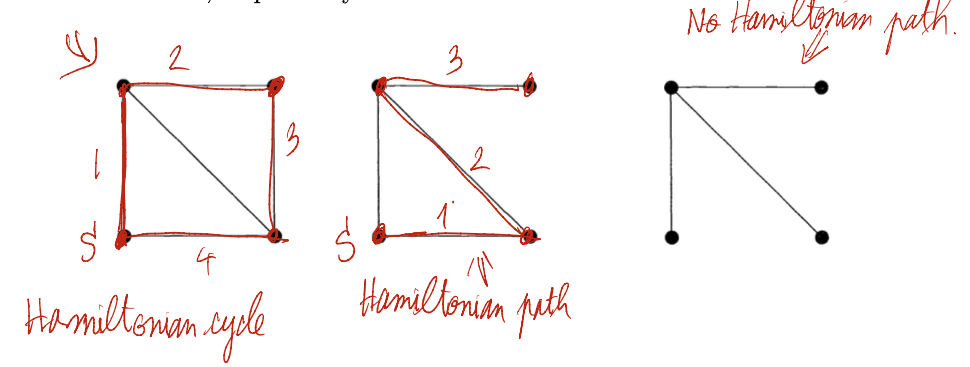
\includegraphics[width=0.95\textwidth]{figures/l03/hamiltonian-graphs}
  \end{center}
  \caption{(Left to right) Hamiltonian, semi-Hamiltonian, and non-Hamiltonian
  Graphs}\label{fig:hamiltonian-graphs-examples}
\end{figure}

\begin{theorem}[Ore, 1960]
  If \(G\) is a simple graph with \(n (\geq 3)\) vertices, and if 
  \[ \deg u + \deg v \geq n \]
  for each pair of non-adjacent vertices \(u\) and \(v\), then \(G\) is
  Hamiltonian.
\end{theorem}

\begin{corollary}[Dirac, 1952]
  If \(G\) is a simple graph with \(n (\geq 3)\) vertices, and if \(\deg v \geq
  n/2\) for each vertex \(v \in V(G)\), then \(G\) is Hamiltonian.
\end{corollary}
